\documentclass[11pt]{amsart}
\usepackage[margin=1.1in]{geometry}
\usepackage{amssymb,booktabs,xcolor,graphicx,tikz}
\usetikzlibrary{arrows.meta,positioning,calc}
\usepackage[colorlinks,urlcolor=blue,citecolor=blue,linkcolor=blue]{hyperref}
\newtheorem{theorem}{Theorem}
\newtheorem{lemma}[theorem]{Lemma}
\newtheorem{proposition}[theorem]{Proposition}
\newtheorem{corollary}[theorem]{Corollary}
\theoremstyle{definition}
\newtheorem{definition}[theorem]{Definition}
\theoremstyle{remark}
\newtheorem{remark}[theorem]{Remark}
% draft markers: everything in red is still to be filled in or confirmed before submission
\newcommand{\todo}[1]{\textcolor{red}{[\textbf{TODO:} #1]}}
\newcommand{\R}{\mathbb R}
\newcommand{\Z}{\mathbb Z}
\newcommand{\low}{\mathrm{low}}
\newcommand{\high}{\mathrm{high}}
\newcommand{\gap}{\mathrm{gap}}
\newcommand{\opt}{\mathrm{opt}}

\title{$k^2-5$ unit squares need a square of side $k$ for every $k\ge7$}
\author{Mohsen Khalili}
\address{Independent researcher}
\email{mkhalili63@yahoo.com}
\author{Sara Gharabaghi}
\address{Independent researcher}
\date{Draft, November 13, 2026}

\begin{document}
\begin{abstract}
Let $s(n)$ be the side of the smallest square into which $n$ unit squares with pairwise disjoint interiors can be
packed, rotations allowed. We prove $s(k^2-5)=k$ for every $k\ge7$. The cases $k=7,8,9$ are known
certificates (ours for $s(44)=7$, Hosono's for $s(59)=8$, Greff's for $s(76)=9$). For all $k\ge10$ at once we give
one family of measures $\mu_k$ on $[0,k]^2$: a fixed corner module in each corner, a wall pattern of depth $4$ that
repeats with period $1$ along each side, and Lebesgue measure in the middle. Its total mass is $k^2-4D$ with
$D=1340566927759/10^{12}>5/4$, and a locality argument reduces the covering property for every $k\ge10$ to a single
$11\times11$ board. That board is checked by Daniel's interval checker \texttt{zmx2} everywhere except near
\emph{tight tiles}: axis-parallel unit squares next to a wall whose mass is exactly $1$, which no box-subdivision
checker can close. For those we prove a Tight-Tile Lemma by an exact blow-up argument: in coordinates scaled by the
tilt, the mass is bounded below on each cell by a concave function built from exact limit values and
interval-certified derivative bounds, and this bound is checked at the cell's vertices in rational arithmetic.
\end{abstract}
\maketitle

\section{Introduction}

Write $s(n)$ for the side of the smallest square containing $n$ unit squares with pairwise disjoint interiors,
each free to rotate. Since $s(k^2)=k$ and $s$ is nondecreasing, $s(n)\le k$ for $(k-1)^2<n\le k^2$, and one asks how
many squares can be removed from the $k\times k$ grid before a smaller container suffices. Friedman's
survey~\cite{friedman} records the history. Nagamochi~\cite{nagamochi} studied $s(k^2-1)$ and $s(k^2-2)$;
Karaku\c{s}~\cite{karakus} later gave a complete proof of $s(k^2-1)=k$, filling a gap in the argument for
Nagamochi's Lemma~1. The family $s(k^2-3)=k$ is due to Kearney and Shiu for $k=3$~\cite{kearney}, Bentz for
$4\le k\le7$~\cite{bentz,bentz2}, and Daniel for all $k\ge6$~\cite{daniel}; since $s$ is nondecreasing, it also gives
$s(k^2-2)=k$ for $k\ge3$. Daniel also proved $s(k^2-4)=k$ for all $k\ge5$ by computer-assisted weighted covers (the
case $k=9$ was first proved by Hosono; see the record in~\cite{daniel}). Ryu's preprint~\cite{ryu} shows that for
every fixed integer $a\ge1$, $s(k^2-a)=k$ for all sufficiently large $k$; its explicit bound reaches $a=5$ only for
$\log k\ge182$, so it does not settle any case covered here.

\begin{theorem}\label{thm:main}
$s(k^2-5)=k$ for every integer $k\ge7$.
\end{theorem}

The upper bound $s(k^2-5)\le k$ is the $k\times k$ grid with five cells empty. The lower bound comes from four
sources:

\begin{center}
\begin{tabular}{llll}
\toprule
$k$ & $n=k^2-5$ & proof of $s(n)\ge k$ & record \\
\midrule
$7$ & $44$ & our weighted cover~\cite{s44} & T-252 of~\cite{squares} \\
$8$ & $59$ & Hosono's weighted cover~\cite{hosono59} & T-066 of~\cite{squares} \\
$9$ & $76$ & Greff's weighted cover~\cite{greff76} & T-184 of~\cite{squares} \\
$\ge10$ & $95,116,\dots$ & the family of this paper & --- \\
\bottomrule
\end{tabular}
\end{center}

\noindent The case $k=10$, $s(95)=10$, was proved earlier by Greff with a single certificate (together with
$s(96)=10$~\cite{greff95}, T-191 of~\cite{squares}); our family gives an independent proof, so the argument does not
depend on it. The bound $k\ge7$ cannot be lowered to all $k$: for $k=3$ and $k=4$, removing five squares does free
space, since $s(4)=2$ and $s(11)<3.88$~\cite{friedman}. The cases $k=5,6$ ($n=20,31$) remain open; covers of the kind
used here very likely cannot reach them (Remark~\ref{rem:small}). Since $s$ is nondecreasing, Theorem~\ref{thm:main} also gives $s(k^2-a)=k$ for
$a=1,\dots,4$ and every $k\ge7$; those cases were already known.

\smallskip
\noindent\textbf{What is new.} Daniel's families for $k^2-3$ and $k^2-4$ already have the corner-plus-periodic-wall
form, and our search reuses his linear program and his checkers. Two things are new. First, the parameters (corner
size $4$, wall depth $4$, element pitch $1/10$, a Lebesgue interior) push the saving per corner from about $1.25$, the
limit Daniel found at pitch $1/5$, to $D\approx1.3406>5/4$. Second, this margin forces the cover to be exactly
tight on many wall tiles, where the existing box-subdivision checkers stall; Section~\ref{sec:tt} gives a rigorous
argument that closes them.

\smallskip
\noindent\textbf{The idea in one paragraph.} A measure on $[0,k]^2$ that gives every unit square mass at least $1$ shows
that at most its total mass of pairwise disjoint unit squares fit (Section~\ref{sec:prelim}). Lebesgue measure has total
$k^2$; we lower this by more than $5$ by working near the walls and corners. Our measure $\mu_k$ is Lebesgue measure in
the middle, a periodic pattern of weighted segments along each wall, and a fixed pattern in each corner
(Figure~\ref{fig:family}). Each corner saves $D\approx1.3406$, so the total is $k^2-4D<k^2-5$. Because the
pattern is periodic, checking that every unit square gets mass at least $1$ for every $k\ge10$ reduces to one board,
$k=11$. Most of that board is checked by an existing interval checker; the hard part is a family of squares next to
the walls that get mass exactly $1$ in the limit of zero tilt, for which we prove a separate lemma.

\smallskip
\noindent\textbf{Structure of the proof.} Section~\ref{sec:prelim} recalls the standard reduction from packings to
weighted covers. Section~\ref{sec:family} defines the family $\mu_k$ and computes its mass, and
Section~\ref{sec:reduction} shows that validity of the single measure $\mu_{11}$ implies the lower bound for every
$k\ge10$. Section~\ref{sec:valid} proves that $\mu_{11}$ is valid (Theorem~\ref{thm:valid}), using the Tight-Tile
Lemma (Theorem~\ref{thm:tt}), which is proved in Section~\ref{sec:tt}. The proof of Theorem~\ref{thm:main} is
assembled at the end of Section~\ref{sec:valid}; Figure~\ref{fig:proofmap} shows how the pieces fit together.
Sections~\ref{sec:controls}--\ref{sec:remarks} describe controls, the search, and remarks.

\begin{figure}[ht]
\centering% Figure: how the pieces of the proof fit together
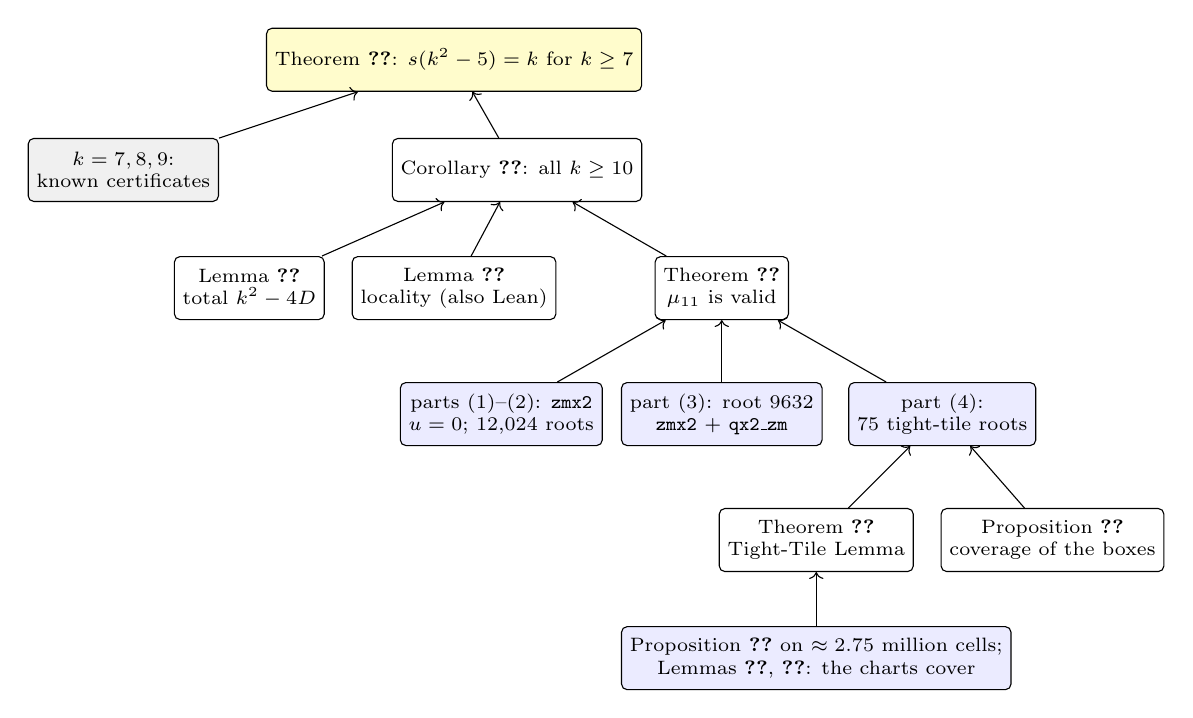
\begin{tikzpicture}[font=\scriptsize,
  box/.style={draw,rounded corners=2pt,align=center,inner sep=3pt,fill=white,minimum height=0.8cm},
  comp/.style={box,fill=blue!8}, ext/.style={box,fill=gray!12}]
  \node[box,fill=yellow!20] (main) at (0,0) {Theorem~\ref{thm:main}: $s(k^2-5)=k$ for $k\ge7$};
  \node[ext] (base) at (-4.2,-1.4) {$k=7,8,9$:\\ known certificates};
  \node[box] (cor) at (0.8,-1.4) {Corollary~\ref{cor:reduce}: all $k\ge10$};
  \node[box] (mass) at (-2.6,-2.9) {Lemma~\ref{lem:mass}\\ total $k^2-4D$};
  \node[box] (loc) at (0,-2.9) {Lemma~\ref{lem:local}\\ locality (also Lean)};
  \node[box] (valid) at (3.4,-2.9) {Theorem~\ref{thm:valid}\\ $\mu_{11}$ is valid};
  \node[comp] (p1) at (0.6,-4.5) {parts (1)--(2): \texttt{zmx2}\\ $u=0$; $12{,}024$ roots};
  \node[comp] (p3) at (3.4,-4.5) {part (3): root $9632$\\ \texttt{zmx2} + \texttt{qx2\_zm}};
  \node[comp] (p4) at (6.2,-4.5) {part (4):\\ $75$ tight-tile roots};
  \node[box] (tt) at (4.6,-6.1) {Theorem~\ref{thm:tt}\\ Tight-Tile Lemma};
  \node[box] (cov) at (7.6,-6.1) {Proposition~\ref{prop:coverage}\\ coverage of the boxes};
  \node[comp] (cells) at (4.6,-7.6) {Proposition~\ref{prop:cell} on $\approx2.75$ million cells;\\ Lemmas~\ref{lem:charts}, \ref{lem:corners}: the charts cover};
  \draw[->] (base) -- (main); \draw[->] (cor) -- (main);
  \draw[->] (mass) -- (cor); \draw[->] (loc) -- (cor); \draw[->] (valid) -- (cor);
  \draw[->] (p1) -- (valid); \draw[->] (p3) -- (valid); \draw[->] (p4) -- (valid);
  \draw[->] (tt) -- (p4); \draw[->] (cov) -- (p4); \draw[->] (cells) -- (tt);
\end{tikzpicture}

\caption{Structure of the proof. Shaded boxes are computations; the others are proved in the text.}
\label{fig:proofmap}
\end{figure}

\section{Preliminaries}\label{sec:prelim}

\subsection*{Notation}
For a point $c\in\R^2$, an angle $\theta$ and $L>0$, let $S(c,\theta,L)$ be the closed square of side $L$ centered at
$c$ whose sides make angle $\theta$ with the axes. A \emph{pose} in $[0,k]^2$ is a closed unit square
$P=S(c,\theta,1)\subseteq[0,k]^2$. Because of the symmetries of the square, $\theta$ matters only modulo $\pi/2$; we
write $u=\tan(\theta/2)$, so that $\theta\in(-\pi/4,\pi/4]$ corresponds to $u\in(-\tan\frac\pi8,\tan\frac\pi8]$.
All measures are finite Borel measures on a square $[0,k]^2$; the \emph{mass} of a pose $P$ is $\mu(P)$.

\subsection*{From packings to covers}
We use the two standard lemmas in the closed form of Daniel~\cite{daniel}, where both are proved in Lean~4
(\texttt{packing\_le\_measure}, \texttt{not\_packs\_of\_measure}); short proofs are also given in our $s(44)$
paper~\cite{s44}.

\begin{lemma}[scaling]\label{lem:scale}
If $n$ unit squares with pairwise disjoint interiors lie in a square of side $L<k$, then there are $n$ pairwise
disjoint poses in $[0,k]^2$.
\end{lemma}

\begin{lemma}[weighted counting]\label{lem:count}
Let $\mu$ be a finite Borel measure on $[0,k]^2$ with $\mu(P)\ge1$ for every pose $P$. Then at most $\mu([0,k]^2)$
poses are pairwise disjoint.
\end{lemma}

\noindent Together: if such a $\mu$ has $\mu([0,k]^2)<n$, then $n$ unit squares do not fit in any square of side
$L<k$ (Lemma~\ref{lem:scale} would give $n$ disjoint poses, contradicting Lemma~\ref{lem:count}), so $s(n)\ge k$.

\begin{definition}
A measure $\mu$ on $[0,k]^2$ is \emph{valid} if $\mu(P)\ge1$ for every pose $P$ in $[0,k]^2$.
\end{definition}

All our measures are finite sums of two kinds of pieces: an axis-parallel segment $\gamma$ carrying a weight
$w>0$ spread uniformly by length (so $\gamma$ itself has mass $w$), and Lebesgue measure on an axis-parallel square.

\section{The family of measures}\label{sec:family}

\begin{figure}[ht]
\centering% Figure: layout of the family measure mu_k (drawn for k = 11; one unit = 0.42 cm)
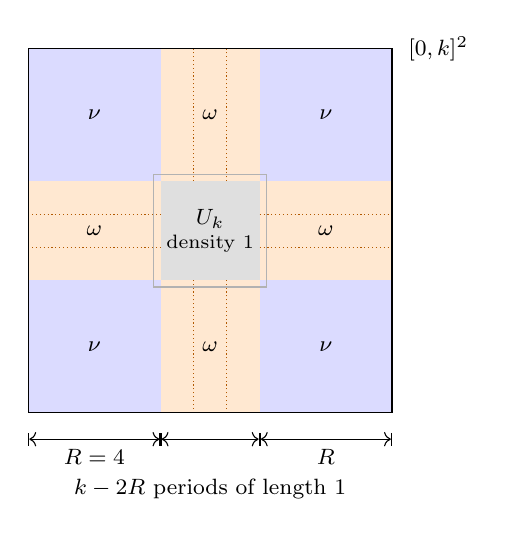
\begin{tikzpicture}[x=0.42cm,y=0.42cm,font=\footnotesize]
  % Lebesgue square U_k
  \fill[gray!25] (3.8,3.8) rectangle (7.2,7.2);
  % corner modules
  \foreach \x/\y in {0/0,7/0,0/7,7/7} \fill[blue!14] (\x,\y) rectangle ++(4,4);
  % wall pieces with their period-1 structure
  \fill[orange!18] (4,0) rectangle (7,4); \fill[orange!18] (4,7) rectangle (7,11);
  \fill[orange!18] (0,4) rectangle (4,7); \fill[orange!18] (7,4) rectangle (11,7);
  \foreach \t in {5,6} {\draw[orange!70!black,densely dotted] (\t,0)--(\t,4); \draw[orange!70!black,densely dotted] (\t,7)--(\t,11);
                        \draw[orange!70!black,densely dotted] (0,\t)--(4,\t); \draw[orange!70!black,densely dotted] (7,\t)--(11,\t);}
  \draw[gray!60] (3.8,3.8) rectangle (7.2,7.2);
  \draw (0,0) rectangle (11,11);
  \node at (2,2) {$\nu$}; \node at (9,2) {$\nu$}; \node at (2,9) {$\nu$}; \node at (9,9) {$\nu$};
  \node at (5.5,2) {$\omega$}; \node at (5.5,9) {$\omega$}; \node at (2,5.5) {$\omega$}; \node at (9,5.5) {$\omega$};
  \node[align=center] at (5.5,5.5) {$U_k$\\[-1pt]\scriptsize density $1$};
  % dimensions
  \draw[|<->|] (0,-0.8) -- node[below] {$R=4$} (4,-0.8);
  \draw[|<->|] (4,-0.8) -- (7,-0.8); \node[below] at (5.5,-1.7) {$k-2R$ periods of length $1$};
  \draw[|<->|] (7,-0.8) -- node[below] {$R$} (11,-0.8);
  \node[right] at (11.2,11) {$[0,k]^2$};
\end{tikzpicture}

\caption{Layout of $\mu_k$ (drawn for $k=11$). The corner module $\nu$ fills each $R\times R$ corner; the wall
pattern $\omega$, of period $1$ along the wall (dotted lines), fills the four bands between the corners; Lebesgue
measure (grey) covers $U_k=[\frac{19}5,k-\frac{19}5]^2$, which overlaps the inner edge of the bands. Increasing $k$ by
one adds one period to each band and leaves the corners unchanged.}
\label{fig:family}
\end{figure}

Fix $R=4$. All coordinates below are multiples of $1/10$, and all weights are exact rationals.

\begin{definition}\label{def:family}
The family is determined by two finite sums of weighted axis-parallel segments, all with endpoints in
$\frac1{10}\Z^2$:
\begin{enumerate}
\item a \emph{corner module} $\nu$ in $[0,R]^2$, invariant under $(x,y)\mapsto(y,x)$;
\item a \emph{wall period} $\omega_0$ in $[0,1]\times[0,R]$ (first coordinate along the wall, second the distance from
the wall), whose segments start at a first coordinate in $[0,1)$. Its periodic extension
$\omega=\sum_{m\in\Z}\bigl(\omega_0+(m,0)\bigr)$ is invariant under $(x,y)\mapsto(-x,y)$.
\end{enumerate}
For an integer $k\ge2R$, the measure $\mu_k$ on $[0,k]^2$ is the sum of the following pieces:
\begin{itemize}
\item four \emph{corner pieces}: $\nu$ in the corner $[0,R]^2$, and its images in the other three corners under the
symmetries of $[0,k]^2$;
\item four \emph{wall pieces}: the bottom wall piece consists of the segments of $\omega$ that lie in the strip
$R\le x\le k-R$; the other three are its images under the symmetries of $[0,k]^2$;
\item Lebesgue measure on the square $U_k=[\tfrac{19}5,\,k-\tfrac{19}5]^2$.
\end{itemize}
\end{definition}

Since every segment has its endpoints on the grid $\frac1{10}\Z^2$ and the lines $x=R$, $x=k-R$ are grid lines, no
segment crosses them, so ``the segments that lie in the strip'' is unambiguous. By construction, and because $\omega$
is symmetric, $\mu_k$ is invariant under the eight symmetries of $[0,k]^2$; for $k=10,\dots,13$ and $k=20$ this was
also checked in exact arithmetic on the built measures. (The family file records, in its header, the part of $U_k$
that lies in the wall and corner strips as belonging to those pieces; this is bookkeeping and gives the same
$\mu_k$.)

The exact data ($2014$ rational variables) are in the file \texttt{sol\_exact\_family.txt}~\cite{repo}. The measure
$\mu_{11}$ is the file \texttt{sol\_exact\_box11.txt} (SHA-256 \texttt{d259fed5\ldots 12099}): $13{,}244$ weighted
segments with coordinate denominator $10$ and mass denominator $2\cdot10^{12}$, plus Lebesgue measure on
$U_{11}=[19/5,36/5]^2$.

Figure~\ref{fig:board} shows the actual measure $\mu_{11}$.

\begin{figure}[ht]
\centering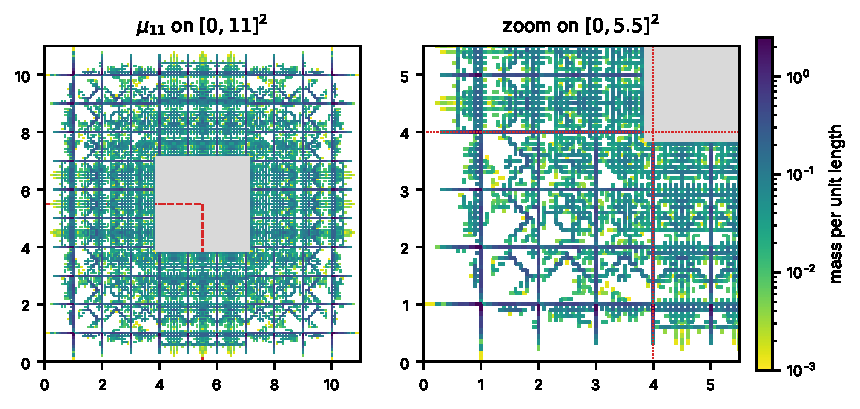
\includegraphics[width=\textwidth]{figures/board.pdf}
\caption{The measure $\mu_{11}$: every segment drawn in a colour given by its mass per unit length (segments lighter
than $10^{-3}$ per unit length are omitted); grey is Lebesgue measure on $U_{11}$. Right: the corner $[0,5.5]^2$; the
dotted red lines are $x=R$ and $y=R$, where the corner module meets the wall bands.}
\label{fig:board}
\end{figure}

\begin{lemma}[mass]\label{lem:mass}
For every integer $k\ge2R$,
\[
\mu_k([0,k]^2)=k^2-4D,\qquad D=\frac{1340566927759}{10^{12}}\approx1.3405669 .
\]
In particular $\mu_k([0,k]^2)<k^2-5$ for every such $k$, since $D>5/4$.
\end{lemma}

\begin{proof}
On each side, the segments of $\omega$ in the strip $R\le x\le k-R$ are the translates $\omega_0+(m,0)$,
$m=R,\dots,k-R-1$, together with the segments of $\omega_0$ on the line $x=0$ translated to $x=k-R$. So the total
mass is
\[
4\,\nu([0,R]^2)+4(k-2R)\,\omega_0([0,1]\times[0,R])+4\,\omega_0(\{0\}\times[0,R])+\Bigl(k-\frac{38}5\Bigr)^2,
\]
a quadratic polynomial in $k$ with leading coefficient $1$. The data are normalized so that it equals $k^2-4D$; this is checked in exact rational arithmetic
from the family file, and independently by building $\mu_k$ for $k=10,11,12,13,20$ and summing all weights. For
$k=11$ the total is $28909433072241/250000000000=121-4D$.
\end{proof}

\noindent Thus $D$ is the saving per corner: away from the corners the measure is as economical as the grid itself.

\section{Reduction to one board}\label{sec:reduction}

The measure $\mu_k$ looks the same, near every point, as $\mu_{11}$ near some point: near a wall it repeats with
period $1$, and near a corner it does not depend on $k$. Since a unit square only sees a window of side $\sqrt2$, its
mass under $\mu_k$ equals the mass of a translated square under $\mu_{11}$ (Figure~\ref{fig:locality}).

\begin{figure}[ht]
\centering% Figure: the three cases of the locality lemma for the first coordinate
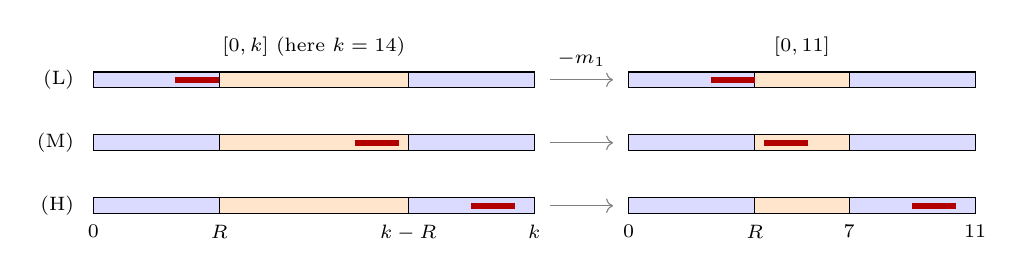
\begin{tikzpicture}[x=0.4cm,y=0.5cm,font=\scriptsize]
  \foreach \row/\lab/\a/\b/\aa/\bb in {0/(L)/2.6/4.0/2.6/4.0, -1.6/(M)/8.3/9.7/4.3/5.7, -3.2/(H)/12.0/13.4/9.0/10.4} {
    \begin{scope}[shift={(0,\row)}]
      \node[left] at (-0.3,0) {\lab};
      \fill[blue!14] (0,-0.2) rectangle (4,0.2); \fill[orange!20] (4,-0.2) rectangle (10,0.2); \fill[blue!14] (10,-0.2) rectangle (14,0.2);
      \draw (0,-0.2) rectangle (14,0.2); \draw (4,-0.2)--(4,0.2) (10,-0.2)--(10,0.2);
      \draw[line width=2pt,red!70!black] (\a,0) -- (\b,0);
      \begin{scope}[shift={(17,0)}]
        \fill[blue!14] (0,-0.2) rectangle (4,0.2); \fill[orange!20] (4,-0.2) rectangle (7,0.2); \fill[blue!14] (7,-0.2) rectangle (11,0.2);
        \draw (0,-0.2) rectangle (11,0.2); \draw (4,-0.2)--(4,0.2) (7,-0.2)--(7,0.2);
        \draw[line width=2pt,red!70!black] (\aa,0) -- (\bb,0);
      \end{scope}
      \draw[->,gray] (14.5,0) -- (16.5,0);
    \end{scope}}
  \node[above] at (7,0.35) {$[0,k]$ (here $k=14$)}; \node[above] at (22.5,0.35) {$[0,11]$};
  \node[above] at (15.5,0.1) {$-m_1$};
  \foreach \x/\l in {0/0,4/R,10/k-R,14/k} \node[below] at (\x,-3.45) {$\l$};
  \foreach \x/\l in {17/0,21/R,24/7,28/11} \node[below] at (\x,-3.45) {$\l$};
\end{tikzpicture}

\caption{The three cases of Lemma~\ref{lem:local} in one coordinate. The red bar is the shadow $[a,b]$ of the unit
square (length at most $\sqrt2$). Blue: within $R$ of a side; orange: the periodic band. Near the left side (L)
nothing moves; in the band (M) an integer shift brings the shadow into $(R,R+1+\sqrt2]$; near the right side (H) the
shadow moves with the side.}
\label{fig:locality}
\end{figure}

\begin{lemma}[locality]\label{lem:local}
Let $k\ge10$. For every pose $P$ in $[0,k]^2$ there is $(m_1,m_2)\in\Z^2$ such that $P'=P-(m_1,m_2)$ is a pose in
$[0,11]^2$ and $\mu_k(P)=\mu_{11}(P')$.
\end{lemma}

\begin{proof}
Let $[a_1,b_1]\times[a_2,b_2]$ be the smallest axis-parallel box containing $P$. Its sides have length
$|\cos\theta|+|\sin\theta|\le\sqrt2$, and $\mu_k(P)$ depends only on the restriction of $\mu_k$ to this box. We
choose $m_1$ from $[a,b]=[a_1,b_1]$ (and $m_2$ from $[a_2,b_2]$ in the same way) by three cases:
\begin{enumerate}
\item[(L)] $a\le R$: take $m_1=0$. Then $b\le R+\sqrt2<5.42$.
\item[(M)] $R<a$ and $b<k-R$: take $m_1=\lceil a\rceil-R-1$, so that $a-m_1\in(R,R+1]$ and
$[a,b]-m_1\subseteq(R,\,R+1+\sqrt2]\subseteq(R,\,7)=(R,\,11-R)$.
\item[(H)] $b\ge k-R$: take $m_1=k-11$. Then $a\ge k-R-\sqrt2>R$ (as $k\ge10$), so case (L) does not apply, and
$[a,b]-m_1\subseteq[11-R-\sqrt2,\,11]$.
\end{enumerate}
The cases are exhaustive, and (L) and (H) are exclusive because $b-a\le\sqrt2<k-2R$.

In each case, every piece of $\mu_k$ that meets the strip $[a,b]\times\R$ coincides, after translation by $m_1$, with
the corresponding piece of $\mu_{11}$ on $([a,b]-m_1)\times\R$, as far as its dependence on $x$ is concerned:
\begin{itemize}
\item In case (L) the strip lies in $\{x<5.42\}$. Pieces attached to the right side of $[0,k]^2$ (right corner
pieces, right wall piece) lie in $\{x\ge k-R\}\subseteq\{x\ge6\}$, and $U_k$ extends to $x=k-\frac{19}5\ge6.2$; so in
this strip $\mu_k$ consists of the left pieces, the segments of the bottom and top wall pieces with $x\le5.42$ (those
of $\omega$ in $R\le x\le5.42$, the same for every $k\ge10$ since $k-R\ge6$), and $U_k$ near its left edge. All of
these are defined relative to the left side $x=0$ in the same way for every $k\ge10$, and in particular for
$\mu_{11}$.
\item In case (M) the strip lies in the open strip $R<x<k-R$, which no corner piece and no left or right wall piece
meets (those lie in $x\le R$ or $x\ge k-R$). There the bottom and top wall pieces coincide with $\omega$ (and its
image), because a segment of $\omega$ that meets the open strip lies in $R\le x\le k-R$; $\omega$ is invariant
under integer translations in $x$; and $U_k$ is invariant under horizontal translation within
$\frac{19}5\le x\le k-\frac{19}5$, which contains the strip. The integer translation by $m_1$ maps the strip into
$R<x<7$, where $\mu_{11}$ has the same description.
\item Case (H) is case (L) reflected in $x\mapsto k-x$ (respectively $x\mapsto11-x$), by the symmetry of $\mu_k$ and
$\mu_{11}$: the strip lies within distance $R+\sqrt2$ of the right side, where both measures are described relative
to that side in the same way.
\end{itemize}
The same holds in $y$ with $m_2$. Each piece of $\mu_k$ is attached either to one side or corner, or is periodic, or is
$U_k$, independently in $x$ and in $y$: a corner piece is attached to two sides, and it meets the box only when the
cases in $x$ and in $y$ are both (L) or (H) for those sides, with zero shift relative to them; a wall piece is attached
to one side in one coordinate and periodic in the other; $U_k$ is a product of two intervals. Therefore the
restriction of $\mu_k$ to $[a_1,b_1]\times[a_2,b_2]$ is the translate by $(m_1,m_2)$ of the restriction of $\mu_{11}$
to $([a_1,b_1]-m_1)\times([a_2,b_2]-m_2)\subseteq[0,11]^2$. Hence $P'=P-(m_1,m_2)$ lies in $[0,11]^2$ and
$\mu_{11}(P')=\mu_k(P)$.
\end{proof}

\begin{remark}[formal proof]\label{rem:lean}
The argument follows Daniel's reduction for $k^2-3$ and $k^2-4$ (file \texttt{BentzFam.lean} in~\cite{daniel}). We
ported it to the $1/10$ grid in Lean~4 (files \texttt{Fam10.lean} and \texttt{Grid10.lean}); the instance proves
\[
\texttt{Valid11}\ \Longrightarrow\ \forall k\ge10,\ s(k^2-5)=k
\]
(theorem \texttt{k2m5\_of\_valid11}), where \texttt{Valid11} states that $\mu_{11}$, read verbatim from the board
file, is valid. It uses only the standard axioms \texttt{propext}, \texttt{Classical.choice} and \texttt{Quot.sound}.
The kernel also checks that the board file is $\mu_{11}$ of the family and that the total mass of $\mu_k$ is
$k^2-4D$ for every $k\ge9$; this was built for the final measure.
As an independent check, a script written from scratch confirms on the $1/10$ grid that every $1.6\times1.6$ window
of $\mu_k$ is an integer translate of a window of $\mu_{11}$ for $k=10,12,13,20$, and it detects a one-weight
mutation of $\mu_{12}$ ($176$ windows fail).
\end{remark}

\begin{corollary}\label{cor:reduce}
If $\mu_{11}$ is valid on $[0,11]^2$, then $s(k^2-5)\ge k$ for every $k\ge10$.
\end{corollary}

\begin{proof}
By Lemma~\ref{lem:local}, $\mu_k$ is valid on $[0,k]^2$ for every $k\ge10$. By Lemma~\ref{lem:mass} its total mass
is $k^2-4D<k^2-5$, so Lemmas~\ref{lem:scale} and~\ref{lem:count} give $s(k^2-5)\ge k$.
\end{proof}

\section{Validity of the $11\times11$ board}\label{sec:valid}

\begin{theorem}\label{thm:valid}
The measure $\mu_{11}$ is valid on $[0,11]^2$: every pose $P$ in $[0,11]^2$ has $\mu_{11}(P)\ge1$.
\end{theorem}

The proof is computer-assisted. Pose space is three-dimensional (the center and the angle). The checker
\texttt{zmx2}~\cite{daniel} splits it into \emph{root boxes} (a grid of initial boxes in center and $u$), subdivides
each root box adaptively, and certifies each sub-box by a rigorous lower bound on the mass of all poses in it. It
computes the geometry in binary64 interval arithmetic with outward rounding and compares masses as exact integers.
In \emph{first-order} mode it also uses the first-order behavior in $u$ near $u=0$. A root box is
\emph{certified} when all of its sub-boxes are, up to a depth cap.

\begin{proof}[Proof of Theorem~\ref{thm:valid}]
The measure $\mu_{11}$ is invariant under the eight symmetries of the square (checked in exact arithmetic), and
these symmetries act on poses. So it suffices to treat poses with center in $[0,\frac{11}2]^2$ and
$u\in[0,\tan\frac\pi8]$. We split this set into four parts.

\begin{enumerate}
\item \textbf{Untilted poses, $u=0$.} The mass of an axis-parallel pose is a piecewise-affine function of its
center whose minimum is attained at finitely many limit points; Daniel's ``Lemma~Z''~\cite{daniel} reduces the check
to these points. Three checks agree that every untilted pose has mass $\ge1$: Lemma~Z at $10{,}000$ one-sided limit
corners in exact arithmetic (minimum exactly $1$, attained at $750$ of them); an independent exact evaluation at
$7{,}717$ corners (minimum exactly $1$); and \texttt{zmx2} in untilted mode on all $2{,}500$ root boxes (all
certified).
\item \textbf{Tilted poses, general position.} \texttt{zmx2} in first-order mode with depth cap $40$ certifies
$12{,}024$ of the $12{,}100$ root boxes. $76$ root boxes remain.
\item \textbf{Root box $9632$.} One remaining root box lies at a corner of $U_{11}$, away from the walls. Its
uncertified sub-boxes are certified by Daniel's exact-rational checker \texttt{qx2\_zm.py}, applied to the
restriction of $\mu_{11}$ to the $3/4$-neighborhood of the root box together with its images under the symmetries.
Concretely, \texttt{zmx2} leaves $6{,}850$ sub-boxes there, all inside the box
$\Omega=[4.3224,4.3264]\times[4.3199,4.3239]\times[0.0229,0.0272]$ in $(x,y,u)$, which lies in a single root box of
\texttt{qx2\_zm.py}. That checker (depth $18$, $2{,}357$ boxes) certifies this root box except $83$ sub-boxes, none of which
meets any of the $6{,}850$; a script checks these containments and disjointness in exact arithmetic. Every pose of
the root box is therefore certified by one of the two checkers. (Removing segments can only lower masses, so a
certificate for the restricted measure is one for $\mu_{11}$.)
\item \textbf{The other $75$ root boxes} are neighborhoods of tight tiles (Section~\ref{sec:tt}). By
Proposition~\ref{prop:coverage}, every sub-box that \texttt{zmx2} leaves uncertified in them is contained, in exact
arithmetic, in the union of the set of poses covered by the Tight-Tile Lemma (Theorem~\ref{thm:tt}) and the set of
untilted poses covered by part (1).
\end{enumerate}
The four parts cover all poses, so every pose has mass at least $1$.
\end{proof}

\begin{proof}[Proof of Theorem~\ref{thm:main}]
The upper bound $s(k^2-5)\le k$ holds because $k^2-5$ unit squares fit in the $k\times k$ grid. For the lower bound,
the cases $k=7,8,9$ are the certificates listed in the introduction~\cite{s44,hosono59,greff76}. For $k\ge10$,
Theorem~\ref{thm:valid} shows that $\mu_{11}$ is valid, and Corollary~\ref{cor:reduce} gives $s(k^2-5)\ge k$.
\end{proof}

\section{The Tight-Tile Lemma}\label{sec:tt}

\subsection{The obstruction}
Take the left wall $x=0$; the other walls follow by symmetry. In the zone $0\le x\le R$ the measure consists of the
left wall piece, which repeats with period $1$ in $y$ for $R\le y\le11-R$, the corner modules near $y=0$ and $y=11$,
and Lebesgue measure on $\frac{19}5\le x\le R$. The \emph{tile} at depth $j\in\{1,2,3\}$ and
height $y$ is the axis-parallel unit square with center $(d_0,y)$, $d_0=j+\frac12$. For the optimal measures of this kind the
mass of such tiles, as a one-sided limit at $u=0$, equals exactly $1$ along whole intervals of $y$: the linear program
pushes these constraints down to equality. We call
these tiles \emph{tight} (Figure~\ref{fig:tile}).

\begin{figure}[ht]
\centering% Figure: a tight tile next to the left wall and a slightly tilted pose near it (tilt exaggerated)
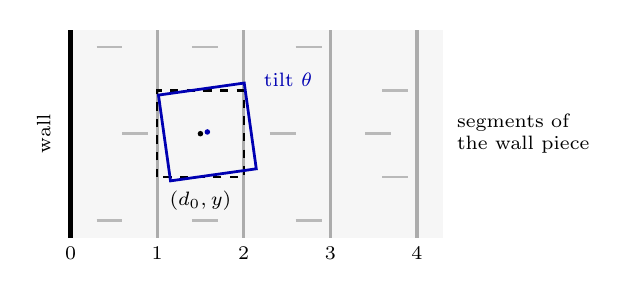
\begin{tikzpicture}[x=1.1cm,y=1.1cm,font=\scriptsize]
  \fill[gray!7] (0,-1.2) rectangle (4.3,1.2);
  \draw[line width=1.5pt] (0,-1.2) -- (0,1.2);
  \node[below] at (0,-1.2) {$0$};
  \foreach \x in {1,2,3,4} {\draw[gray!65,line width=1.1pt] (\x,-1.2) -- (\x,1.2); \node[below] at (\x,-1.2) {$\x$};}
  \foreach \y/\x in {-1/0.3,-1/1.4,-1/2.6,0/0.6,0/2.3,0/3.4,1/0.3,1/1.4,1/2.6,-0.5/3.6,0.5/3.6} \draw[gray!55,line width=0.9pt] (\x,\y) -- ++(0.3,0);
  \draw[dashed,line width=0.9pt] (1,-0.5) rectangle (2,0.5);
  \begin{scope}[shift={(1.58,0.02)},rotate=8]
    \draw[blue!70!black,line width=1pt] (-0.5,-0.5) rectangle (0.5,0.5);
  \end{scope}
  \fill (1.5,0) circle (1pt); \fill[blue!70!black] (1.58,0.02) circle (1pt);
  \node[below] at (1.5,-0.55) {$(d_0,y)$};
  \node[blue!70!black,right] at (2.12,0.62) {tilt $\theta$};
  \node[left,rotate=90,anchor=south] at (-0.12,0) {wall};
  \node[right,align=left] at (4.35,0) {segments of\\the wall piece};
\end{tikzpicture}

\caption{A tight tile at depth $1$ (dashed) and a nearby pose (blue), with the tilt exaggerated. The tile lies
between the lines $x=1$ and $x=2$, which carry segments of the wall piece; in the limit of zero tilt its mass is exactly
$1$. A pose that is shifted by $\delta$ and tilted by $\theta$ gains or loses pieces of segments near its edges at first
order in $\theta$; the lemma shows that the net change is never negative.}
\label{fig:tile}
\end{figure}

A sub-box whose closure contains a tight limit pose can never be certified by a bound of the form ``mass at a point
of the box minus a Lipschitz constant times the box size,'' however small the box is. Of the $76$ root boxes that
\texttt{zmx2} leaves, $75$ are exactly the neighborhoods of tight tiles. The idea of the Tight-Tile Lemma is to
blow up these neighborhoods: in coordinates scaled by the tilt, the mass has an exact limit as the tilt tends to
$0$, and the first-order growth with the tilt can be bounded rigorously.

\subsection{Statement}
Write the center of a pose as $(d_0+\delta,\,y)$ and its angle as $\tan(\theta/2)=\sigma u$ with $\sigma\in\{+1,-1\}$
and $u>0$ (in this section $u$ denotes $|\tan(\theta/2)|$). Let
\[
u_0=\tfrac1{4000},\qquad K=4,\qquad \delta_{\max}=Ku_0=\tfrac1{1000},
\]
and define the height ranges
\begin{align*}
I(3/2)&=[1.4,1.7]\cup[2.4,2.7]\cup[3.3,5.5],\\
I(5/2)&=[1.4,1.7]\cup[2.3,2.7]\cup[3.3,3.7]\cup[3.8,5.5],\\
I(7/2)&=[1.4,1.7]\cup[2.3,2.7]\cup[3.3,3.7]\cup[4.1,4.5].
\end{align*}

\begin{theorem}[Tight-Tile Lemma]\label{thm:tt}
Let $d_0\in\{3/2,5/2,7/2\}$, $\sigma\in\{+1,-1\}$ and $y\in I(d_0)$. Every pose with center $(d_0+\delta,y)$ and
$\tan(\theta/2)=\sigma u$, where $0<u\le u_0$ and $|\delta|\le\delta_{\max}$, has $\mu_{11}$-mass at least $1$. The
same holds with $u_0=1/2000$ and $\delta_{\max}=1/500$ on five further ranges of $y$, each extended by $1/500$ at both
ends: $[4.2,4.3]$ and $[4.5,4.6]$ for $(d_0,\sigma)=(3/2,+1)$; $[3.8,3.9]$ and $[5.4,5.5]$ for $(3/2,-1)$; and
$[4.4,4.5]$ for $(5/2,-1)$.
\end{theorem}

The proof occupies the rest of this section. It is a computer-assisted case analysis in which every step is either
an exact rational computation or a rigorously rounded interval enclosure. The mathematical part of the proof is given in full below:
the exact chord formula, the charts and their covering (Lemma~\ref{lem:charts}), the cell certificate
(Lemma~\ref{lem:concave} and Proposition~\ref{prop:cell}), and the corner zones (Lemma~\ref{lem:corners}). The
computational part, certifying every cell, is done by the program \texttt{ttbox} (about $1{,}000$ lines of Python,
in~\cite{repo}); the technical report~\cite{ttproof} documents the implementation, the rounding rules and the
logs.

\subsection{Exact chords}
Let $N=1+u^2$ and $e_1=\bigl((1-u^2)/N,\,2u/N\bigr)$, $e_2=\bigl(-2u/N,\,(1-u^2)/N\bigr)$, the unit vectors along the
sides of a pose tilted by $\theta$. The pose with center $c$ is $P=\{z\in\R^2:|(z-c)\cdot e_i|\le\frac12,\ i=1,2\}$.
Consider a segment $\gamma=\{g+\tau(g'-g):\tau\in[0,1]\}$ of weight $w$. Each of the four half-planes of $P$ reads
$\tau A\le B$ with
\[
A=\pm\,(g'-g)\cdot Ne_i,\qquad B=\tfrac N2\mp(g-c)\cdot Ne_i ,
\]
for $i=1,2$ and both signs. Let $\mathcal B^+$ consist of $1$ and the ratios $B/A$ with $A>0$ (upper bounds on
$\tau$), and $\mathcal B^-$ of $0$ and the ratios with $A<0$ (lower bounds); constraints with $A=0$ hold either for
all $\tau$ or for none. Then $\gamma$ contributes $w\cdot\max(0,\min\mathcal B^+-\max\mathcal B^-)$ to $\mu(P)$.
The factor $N>0$ does not change the inequalities, and with it $A$ and $B$ are polynomials in $u$ and $c$.

\subsection{Blow-up charts}
The key choice is the scale variable: we always use the tilt, $h=u$. Near a base line $y_b\in\frac1{10}\Z$, with
$t=y-y_b$, the four cases $|\delta|\le Ku$ or not and $|t|\le Ku$ or not give four \emph{charts}, each with two
\emph{face coordinates} $(p,q)$ and a \emph{slab} condition on $h$:

\begin{center}
\begin{tabular}{llll}
\toprule
chart & poses & face coordinates $(p,q)$ & slab \\
\midrule
$C_u$ & $|\delta|,|t|\le Ku$ & $(\delta/u,\ t/u)\in[-K,K]^2$ & $0\le h\le u_0$\\
$W_t$ & $|\delta|\le Ku<|t|$ & $(\delta/u,\ |t|)$ & $h\le|t|/K$\\
$W_d$ & $|t|\le Ku<|\delta|$ & $(t/u,\ |\delta|)$ & $h\le|\delta|/K$\\
$W_{td}$ & $Ku<|\delta|$ and $Ku<|t|$ & $(|t|,|\delta|)$, two triangles & $h\le\min(|t|,|\delta|)/K$\\
\bottomrule
\end{tabular}
\end{center}

\noindent Figure~\ref{fig:zones}(a) shows the four charts at a fixed tilt. Between base lines, where
$Ku_0\le t\le\frac1{10}-Ku_0$, two strip charts are used: $\Sigma_u$ with face
coordinates $(\delta/u,\,y)$ for $|\delta|\le Ku$ and slab $h\le u_0$, and $\Sigma_d$ with face coordinates
$(y,\,|\delta|)$ for $|\delta|>Ku$ and slab $h\le|\delta|/K$.

\begin{lemma}[the charts cover]\label{lem:charts}
Every pose of Theorem~\ref{thm:tt} (with $u_0=1/4000$) lies in one of the charts above, with face coordinates in the
stated ranges and $h=u$ in the stated slab. The same holds for $u_0=1/2000$ on the further ranges.
\end{lemma}

\begin{proof}
Each set $I(d_0)$ is a finite union of intervals $[y_1,y_2]$ with $y_1,y_2\in\frac1{10}\Z$. Every $y$ in such an
interval satisfies either $|y-y_b|\le Ku_0$ for a base line $y_b\in\frac1{10}\Z\cap[y_1,y_2]$, or lies in a strip
$[y_b+Ku_0,\,y_b+\frac1{10}-Ku_0]$ between two consecutive base lines of the interval. Near a base line, put
$t=y-y_b$, so $|t|\le Ku_0$, and $|\delta|\le\delta_{\max}=Ku_0$. Exactly one of four cases holds. If
$|\delta|,|t|\le Ku$, the pose is in $C_u$ with $(p,q)=(\delta/u,t/u)\in[-K,K]^2$ and $h=u\le u_0$. If
$|\delta|\le Ku<|t|$, it is in $W_t$ with $p=\delta/u\in[-K,K]$, $q=|t|\le Ku_0$ and $h=u<|t|/K$. The case
$W_d$ is symmetric. If $Ku<|\delta|$ and $Ku<|t|$, it is in $W_{td}$ with $h<\min(|t|,|\delta|)/K$. In a strip, the
same split by $|\delta|\le Ku$ or $>Ku$ gives $\Sigma_u$ or $\Sigma_d$. For the five further ranges, with
$u_0=1/2000$, the line charts of the two end lines reach $1/500=Ku_0$ beyond the range. \end{proof}

In each chart the center is $c_0+h\,c_1$, with $c_0$ affine in $(p,q)$ and $c_1$
polynomial in $(p,q,h)$, so $A$ and $B$ are polynomials in $(p,q,h)$ with rational coefficients. Common powers of
$h>0$ are divided out exactly. In the limit $h\to0$ each ratio $B/A$ becomes \emph{affine} in $(p,q)$; this is what
makes the tight tiles tractable.

\begin{figure}[ht]
\centering% Figure: the four-way splits. (a) charts near a base line in the (delta, t) plane at a fixed tilt u;
% (b) the zones around a corner point of a face; (c) wedge-corner zones and the ray zones.
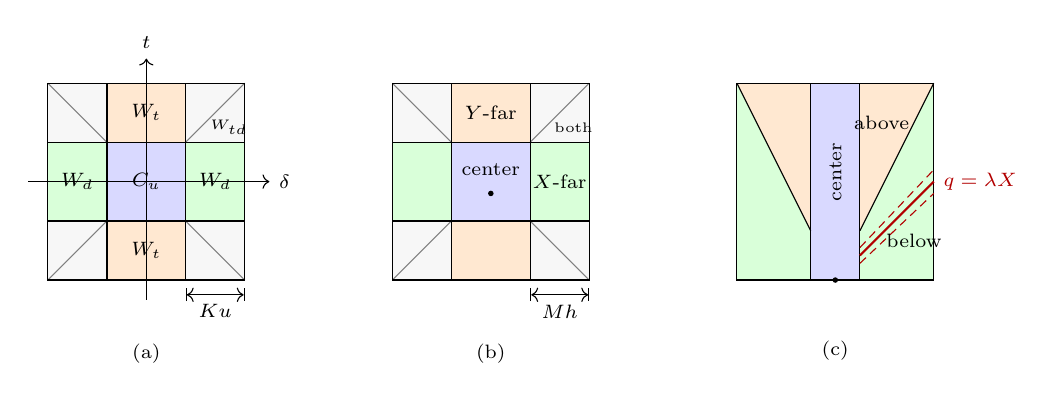
\begin{tikzpicture}[font=\scriptsize,x=1.25cm,y=1.25cm]
 \def\ttfourway{%
  \fill[gray!6] (-1,-1) rectangle (1,1);
  \fill[blue!15] (-0.4,-0.4) rectangle (0.4,0.4);
  \fill[orange!18] (-0.4,0.4) rectangle (0.4,1); \fill[orange!18] (-0.4,-1) rectangle (0.4,-0.4);
  \fill[green!15] (0.4,-0.4) rectangle (1,0.4); \fill[green!15] (-1,-0.4) rectangle (-0.4,0.4);
  \foreach \sx in {1,-1} \foreach \sy in {1,-1} \draw[gray] (0.4*\sx,0.4*\sy) -- (\sx,\sy);
  \draw (-1,-1) rectangle (1,1); \draw (-0.4,-1) -- (-0.4,1) (0.4,-1) -- (0.4,1) (-1,-0.4) -- (1,-0.4) (-1,0.4) -- (1,0.4);}
 \begin{scope}
  \ttfourway
  \node at (0,0) {$C_u$}; \node at (0,0.7) {$W_t$}; \node at (0,-0.7) {$W_t$}; \node at (0.7,0) {$W_d$}; \node at (-0.7,0) {$W_d$};
  \node[font=\tiny] at (0.84,0.55) {$W_{td}$};
  \draw[->] (-1.2,0) -- (1.25,0) node[right] {$\delta$}; \draw[->] (0,-1.2) -- (0,1.25) node[above] {$t$};
  \draw[|<->|] (0.4,-1.15) -- node[below] {$Ku$} (1,-1.15);
  \node at (0,-1.75) {(a)};
 \end{scope}
 \begin{scope}[shift={(3.5,0)}]
  \ttfourway
  \node at (0,0.12) {center}; \node at (0,0.7) {$Y$-far}; \node at (0.7,0) {$X$-far}; \node[font=\tiny] at (0.84,0.55) {both};
  \fill (0,-0.12) circle (1pt);
  \draw[|<->|] (0.4,-1.15) -- node[below] {$Mh$} (1,-1.15);
  \node at (0,-1.75) {(b)};
 \end{scope}
 \begin{scope}[shift={(7.0,-1)},y=2.5cm]
  \fill[gray!6] (-1,0) rectangle (1,1);
  \fill[blue!15] (-0.25,0) rectangle (0.25,1);
  \fill[green!15] (0.25,0) -- (1,0) -- (1,1) -- (0.25,0.25) -- cycle; \fill[green!15] (-0.25,0) -- (-1,0) -- (-1,1) -- (-0.25,0.25) -- cycle;
  \fill[orange!18] (0.25,0.25) -- (1,1) -- (0.25,1) -- cycle; \fill[orange!18] (-0.25,0.25) -- (-1,1) -- (-0.25,1) -- cycle;
  \draw (-1,0) rectangle (1,1); \draw (-0.25,0) -- (-0.25,1) (0.25,0) -- (0.25,1);
  \draw (0.25,0.25) -- (1,1) (-0.25,0.25) -- (-1,1);
  \draw[red!70!black,thick] (0.25,0.125) -- (1,0.5);
  \draw[red!70!black,densely dashed] (0.25,0.085) -- (1,0.44) (0.25,0.165) -- (1,0.56);
  \node[rotate=90] at (0,0.55) {center};
  \node at (0.47,0.8) {above}; \node at (0.8,0.2) {below};
  \node[red!70!black,right] at (1,0.5) {$q=\lambda X$};
  \fill (0,0) circle (1pt);
  \node at (0,-0.36) {(c)};
 \end{scope}
\end{tikzpicture}

\caption{The case splits, drawn at a fixed value of the scale $h=u$. (a) The four charts near a base line, in the
plane of the offsets $(\delta,t)$: $C_u$ where both offsets are at most $Ku$, $W_t$ and $W_d$ where one of them is
larger, $W_{td}$ (two triangles each) where both are. As $u\to0$ the central square shrinks, and the coordinates
$\delta/u$, $t/u$ keep it of fixed size. (b) The same split one level down, around a corner point $(p^*,q^*)$ of a
face, with scale $Mh$. (c) The zones around a corner point on the edge $q=0$ of a wedge chart, and the near zone
(dashed) around a ray $q=\lambda X$, $X=|p-p^*|$.}
\label{fig:zones}
\end{figure}

\subsection{The cell bound}
A \emph{cell} is a set $Z=\{(p,q,h):(p,q)\in\Pi,\ \low(p,q)\le h\le\high(p,q)\}$, where $\Pi$ is a convex polygon
with rational vertices and $0\le\low\le\high$ are affine functions. Since $Z$ is convex, its vertices are among the
points $(v,\low(v))$ and $(v,\high(v))$ for vertices $v$ of $\Pi$. Let $\mathrm{Bx}(Z)$ be the box
$\mathrm{bbox}(\Pi)\times[0,\max\high]$.

On a cell, every constraint $\tau A\le B$ is classified by outward-rounded interval arithmetic on $\mathrm{Bx}(Z)$
as \emph{regular} ($A$ has constant sign, so $B/A$ is $C^1$), \emph{inactive} ($B\ge\max(0,A)$, so it holds for all
$\tau\in[0,1]$), or \emph{empty} ($B<\min(0,A)$, so it fails for all $\tau$ and the chord is $0$). On charts of wedge
shape, where $h\le\chi\,\xi$ for a nonnegative face coordinate $\xi$ and a constant $\chi>0$, the last two
tests are made after the exact substitution $h=\eta\,\xi$ with $\eta\in[0,\chi]$ and division by the largest
power of $\xi$; near the apex of a wedge, a second substitution expresses one face coordinate as a bounded multiple
$\zeta$ of the other. If the auxiliary variables $\eta,\zeta$ make an interval test inconclusive, their ranges are
bisected, and the same verdict is required on every piece. For a regular constraint we further require that
$A(p,q,0)$ is a nonzero constant and $B(p,q,0)$ is affine. A cell on which some constraint fits none of these cases
is split.

For each segment, write $b_r^+=B/A$ for its regular constraints with $A>0$ together with the constant bound $1$, and
$b_r^-=B/A$ for those with $A<0$ together with the constant bound $0$ (a constant bound has derivative $0$; inactive
constraints are dropped, and a segment with an empty constraint contributes $0$ on the whole cell). These have affine
\emph{limit values} $b_r^\pm(0)$ on $\Pi$. The polygon is split
exactly so that, on all of $\Pi$, the minimizing upper bound $b_{r_*}^+$, the maximizing lower bound $b_{r_*}^-$ and
the sign of the limit chord $f(0)=b^+_{r_*}(0)-b^-_{r_*}(0)$ are fixed. Let
\[
\alpha_r\le\inf_{\mathrm{Bx}(Z)}\partial_h b_r^+,\qquad \beta_r\ge\sup_{\mathrm{Bx}(Z)}\partial_h b_r^-
\]
be interval enclosures of the derivative $\partial_h(B/A)=(A\,\partial_hB-B\,\partial_hA)/A^2$. Since the vertical
segment $\{(p,q)\}\times[0,h]$ lies in $\mathrm{Bx}(Z)$ for every point of $Z$, the mean value theorem gives
\[
b_r^+(h)\ge b_r^+(0)+h\,\alpha_r,\qquad b_r^-(h)\le b_r^-(0)+h\,\beta_r .
\]
This is the Lipschitz condition, made explicit and uniform on the cell.

In words: in the limit $h\to0$ every chord is an exact affine function of the face coordinates, and for $h>0$ each
endpoint of a chord moves at most linearly in $h$, at a rate bounded rigorously on the whole cell. The next lemma turns
these two facts into a lower bound for the chord that is concave, so that it only has to be checked at the vertices of
the cell.

\begin{lemma}\label{lem:concave}
Let $\gap^+_r=b_r^+(0)-b_{r_*}^+(0)\ge0$ and $\gap^-_r=b_{r_*}^-(0)-b_r^-(0)\ge0$, and
\[
\varphi=\min_r(\gap^+_r+h\,\alpha_r)+\min_r(\gap^-_r-h\,\beta_r).
\]
Then $\varphi$ is concave in $(p,q,h)$, and the chord $\ell(h)=\max\bigl(0,f(h)\bigr)$, where
$f(h)=\min\mathcal B^+-\max\mathcal B^-$, satisfies $\ell(h)-\ell(0)\ge\max(\opt_0,\opt_1)$ with
\begin{itemize}
\item $\opt_0=\varphi$ and $\opt_1=-f(0)$ if $f(0)\ge0$ on $\Pi$;
\item $\opt_0=f(0)+\varphi$ and $\opt_1=0$ if $f(0)\le0$ on $\Pi$.
\end{itemize}
Every convex combination $\kappa\,\opt_1+(1-\kappa)\,\opt_0$ with $\kappa\in[0,1]$ is concave and is also a lower
bound for $\ell(h)-\ell(0)$.
\end{lemma}

\begin{proof}
$\varphi$ is a sum of minima of affine functions, hence concave. By the mean value bounds,
$\min\mathcal B^+(h)\ge b^+_{r_*}(0)+\min_r(\gap^+_r+h\alpha_r)$ and similarly for $\max\mathcal B^-(h)$, so
$f(h)\ge f(0)+\varphi$. If $f(0)\ge0$, then $\ell(0)=f(0)$, so $\ell(h)-\ell(0)\ge f(h)-f(0)\ge\varphi$ and
$\ell(h)-\ell(0)\ge-\ell(0)=-f(0)$. If $f(0)\le0$, then $\ell(0)=0$, and $\ell(h)\ge f(h)\ge f(0)+\varphi$ and
$\ell(h)\ge0$. A convex combination of two lower bounds is at most their maximum, and a convex combination of
concave functions is concave.
\end{proof}

\begin{proposition}[cell certificate]\label{prop:cell}
On a cell $Z$, let $G(p,q)$ be the limit value of $\mu_{11}(P)-1$ as $h\to0$, which is exactly affine on $\Pi$, except
that for the depth-$7/2$ tiles the Lebesgue part is replaced by its affine McCormick lower bound described below, let $\kappa_i\in[0,1]$ be
rational numbers, one per segment $i$ of weight $w_i$, and let
\[
T=G+\sum_i w_i\bigl(\kappa_i\,\opt_{1,i}+(1-\kappa_i)\,\opt_{0,i}\bigr)+h\,\alpha_U ,
\]
where $\alpha_U$ is a lower bound for the $h$-derivative of the Lebesgue term on $\mathrm{Bx}(Z)$. Then
$\mu_{11}(P)-1\ge T$ on $Z$, and $T$ is concave. Hence if $T\ge0$ at the vertices of $Z$, evaluated in exact
rational arithmetic, then $\mu_{11}(P)\ge1$ for every pose $P$ in $Z$.
\end{proposition}

\begin{proof}
The mass is the sum of the segment contributions $w_i\ell_i$ and the Lebesgue term, so the first claim follows from
Lemma~\ref{lem:concave} and the derivative bound for the Lebesgue term described below. A concave function on a
polytope attains its minimum at a vertex.
\end{proof}

The coefficients $\kappa_i$ are proposed by a floating-point linear program and then used as exact rationals; the
linear program plays no role in soundness. Only the depth-$7/2$ tiles reach $U_{11}$. For them, the limit value of
the area $|P\cap U_{11}|$ is a product of two clamped affine functions; it is bounded below by its McCormick
envelope after splitting $\Pi$ at the kinks. Its $h$-derivative is the integral of the normal velocity of $\partial P$
over $\partial P\cap U_{11}$; each edge of $P$ is clipped against $U_{11}$ like a segment, and the integral is enclosed
by intervals.

A cell that fails is split, by bisection or along a \emph{kink plane} $h=-f(0)/\dot f$, where a segment's bound changes
branch ($\dot f$ being the slope in $h$ of its bound), down to a side length of $2^{-30}$. A cell still refused at that size is
reported as a failure, never discarded.

\subsection{Corner points}
At isolated points of a face two events coincide, for instance two edges of the tilted square crossing segment
endpoints at the same time; there the bound fails at every scale on the cells that touch the point. These points
have rational face coordinates $(p^*,q^*)$ with small denominators. The checker groups the refused cells by such a point, takes the smallest dyadic
$\rho$ for which the box $[p^*-\rho,p^*+\rho]\times[q^*-\rho,q^*+\rho]$ contains them all, and re-covers that box
by a second blow-up, again with scale $h$. Write $X=|p-p^*|$, $Y=|q-q^*|$ and $M=4$.

\begin{center}
\begin{tabular}{llll}
\toprule
zone & poses & face coordinates & slab \\
\midrule
center & $X,Y\le Mh$ & $(\bar p,\bar q)\in[-M,M]^2$, $(p,q)=(p^*,q^*)+h(\bar p,\bar q)$ & $h\le u_0$\\
$X$-far & $X>Mh\ge Y$ & $(X,\bar q)$, $q=q^*+h\bar q$ & $h\le X/M$\\
$Y$-far & $Y>Mh\ge X$ & $(\bar p,Y)$, $p=p^*+h\bar p$ & $h\le Y/M$\\
both far & $X,Y>Mh$ & $(X,Y)$, two triangles & $h\le\min(X,Y)/M$\\
\bottomrule
\end{tabular}
\end{center}

\noindent (each far zone for both signs of $p-p^*$ and $q-q^*$). In a wedge chart, with slab $h\le q/K$, the
corner points lie on the edge $q=0$, the box is $[p^*-\rho,p^*+\rho]\times[0,\rho]$, and there are three zones:
center ($X\le Mh$, face $(\bar p,q)$ with $p=p^*+h\bar p$, slab $h\le q/K$); far, above the diagonal ($X>Mh$,
$q\ge X$, slab $h\le X/M$); and far, below the diagonal ($X>Mh$, $q\le X$, slab $h\le q/K$). Where it was needed (two corners in each of two jobs), the last zone is covered once more by five zones around a ray $q=\lambda X$ through the corner
point ($\lambda=1/2$): with $\Delta=q-\lambda X$ and $M'=1$, a near zone $|\Delta|\le M'h$ (face $(X,(q-\lambda X)/h)$, slab
$h\le\lambda X/(K-M')$), and on each side of the ray a zone where $|\Delta|>M'h$ with slab $h\le|\Delta|/M'$ and a zone
where the original slab $h\le q/K$ is kept, split where $|\Delta|/M'=q/K$.

\begin{lemma}[the corner zones cover]\label{lem:corners}
Each family of zones covers the set of poses it replaces: the box times the slab of the original chart. (For the
first family, $\rho\le Mu_0$ is required, and checked by the program.)
\end{lemma}

\begin{proof}
For the first family, every pose satisfies exactly one of $X\le Mh$ or $X>Mh$, and one of $Y\le Mh$ or $Y>Mh$. In
the center zone $(\bar p,\bar q)=((p-p^*)/h,(q-q^*)/h)\in[-M,M]^2$ and $h\le u_0$ is the original slab. In the far
zones the defining strict inequalities give the slab bounds, which are at most $\rho/M\le u_0$. For the wedge
corners, a pose with $X\le Mh$ is in the center zone with $\bar p\in[-M,M]$ and the original slab; a pose with $X>Mh$
and $q\ge X$ has $h<X/M$; a pose with $X>Mh$ and $q\le X$ keeps $h\le q/K$. For the ray zones, take a pose with
$h\le q/K$. If $|\Delta|\le M'h$, then $q\le\lambda X+M'h$, and $Kh\le q$ gives $h\le\lambda X/(K-M')$. If $\Delta>M'h$,
then $h<\Delta/M'$, and the pose lies in the zone with that slab when $\Delta/M'\le q/K$, and in the zone that keeps
$h\le q/K$ otherwise. The case $-\Delta>M'h$ is the same. Some zones contain more poses than needed; that is harmless,
because the pose formulas are polynomial identities and Proposition~\ref{prop:cell} is proved on each zone as a
whole.
\end{proof}

All zones are again charts in the sense above: the center of the pose is polynomial in the face coordinates and $h$,
so they are certified by Proposition~\ref{prop:cell}.

\subsection{Computation}
The poses of Theorem~\ref{thm:tt} are split into $308$ jobs at $u_0=1/4000$, one per base line or strip, depth and
tilt sign, and $15$ more at $u_0=1/2000$. Each job reports every chart and every corner zone. In total about $2.75$
million cells were certified. Two jobs, at depth $7/2$ and $y_b=3.5$, needed the wedge-corner and ray zones; one job
at $u_0=1/2000$ needed four corner boxes. Every chart and every corner zone of every job is certified, with no
refused cell. This proves Theorem~\ref{thm:tt}.

\subsection{Coverage of the remaining boxes}\label{sec:coverage}

\begin{proposition}\label{prop:coverage}
Every sub-box that \texttt{zmx2} leaves uncertified in the $75$ tight-tile root boxes consists of poses covered by
Theorem~\ref{thm:tt} or of untilted poses.
\end{proposition}

\begin{proof}
\texttt{zmx2} was rerun on these root boxes with the same settings, printing all $1{,}255{,}023$ uncertified
sub-boxes, which have exact rational ends in center and $u$. A sub-box near $x=d_0$ consists of left-wall tile poses
with $\sigma=+1$. A sub-box near $y=d_0$ is mapped to left-wall poses by the reflection $(x,y)\mapsto(y,x)$, which
preserves $\mu_{11}$ and reverses orientation, so $\sigma=-1$ and the height is the original $x$. A script checks in exact arithmetic that every sub-box
satisfies $u\le u_0$, has offset at most $\delta_{\max}$ from $d_0$, and lies in the certified height ranges (for $u\le1/2000$ also the five further ranges with their extensions); its
points with $u=0$ are untilted. The same script re-reads every job output and requires each expected chart to be
present, run with the stated parameters and free of refused cells. All $1{,}255{,}023$ sub-boxes pass, and all $308$ jobs at $u_0=1/4000$ and all $15$ at
$u_0=1/2000$ pass the job check.
\end{proof}

\section{Controls and independent checks}\label{sec:controls}

The controls below are not part of the proof. They test the checkers: a checker that never refuses proves
nothing. Each control runs a deliberately \emph{modified} measure, not $\mu_{11}$, through a checker on a region
where $\mu_{11}$ itself is certified, and the checker must refuse it.
\begin{itemize}
\item \texttt{zmx2}, at depth $24$ on the root box $(15,36)$ of the final measure, certifies $\mu_{11}$ ($0$ uncertified
sub-boxes) and refuses the measures with every segment weight multiplied by $0.999$ ($209$ uncertified) and by
$0.993$ ($217$).
\item \texttt{qx2\_zm.py} on the root box of part (3) of Theorem~\ref{thm:valid}, with every segment weight multiplied by
$0.999$, leaves $87$ sub-boxes uncertified (against $83$ for $\mu_{11}$), and three of them meet sub-boxes that
\texttt{zmx2} leaves; so the closure argument of part (3) fails for the modified measure, as it must.
\item The tight-tile checker refuses three modified measures on regions where $\mu_{11}$ is certified: all weights
multiplied by $0.99$; the segments on the line $x=2$ weakened by $1\%$; and the subtlest one, a measure with the
\emph{same} limit values as $\mu_{11}$ but a smaller first-order growth. It is built from $\mu_{11}$ by moving one
segment ($x=1.9$, $y\in[5.0,5.1]$, weight $0.0142$), which touches the tile centered at $(3/2,9/2)$ only at a
point, to $y\in[5.1,5.2]$. This changes no limit value at that tile, but the modified measure is no longer valid:
the pose with center $(3/2+h,\,9/2+h)$ and $u=h$ has exact mass $1-1.34\cdot10^{-7}$ at $h=10^{-6}$, while under
$\mu_{11}$ the same pose has mass $1+1.22\cdot10^{-7}$. A checker that looked only at limit values could not tell the
two measures apart. On the same region of the face, the tight-tile checker certifies $\mu_{11}$ with no refused cell
($155$ cells processed), and refuses $1{,}190$ of the $6{,}079$ cells it processes for the modified measure, including
those containing the violating poses. So it detects
first-order deficits, as the proof requires.
\item An independent review of the tight-tile proof and code recomputed $\mu_{11}(P)-1$ in exact rational
arithmetic, with all $13{,}244$ segments and the exact area of $P\cap U_{11}$, at every vertex of every certified cell
in sample regions, including all corner and ray zones, and found $T\le\mu_{11}(P)-1$ throughout. It also tested the
interval arithmetic at $44{,}000$ adversarial points and sampled the covering case analyses exactly, with no
failures.
\item A floating-point evaluation of $\mu_{11}$, written from scratch, at $90{,}000$ random, $90{,}000$ near-tile and
$90{,}000$ near-$45^\circ$ poses found no mass below $1$ beyond rounding ($1-9\cdot10^{-15}$, in the Lebesgue
middle, where the mass is exactly $1$).
\end{itemize}

\section{How the measure was found}\label{sec:search}

This section is not part of the proof.

We minimized $\mu_k([0,k]^2)$ over the family by Daniel's quadrant linear program \texttt{qx2\_lp.py}~\cite{daniel}:
segment variables on the $1/10$ grid with $R=4$, exact rows for the limits $\theta\to0$, and a tilt margin (mass at
least $1+0.05\,\min(\theta,\pi/180)\,(1-|P\cap U_k|)$, $\theta$ in radians), so that the checkers have room away from tight poses.
Each round projects the linear-programming solution to an exact rational point on its tight rows (by QR pivoting
and exact solution with FLINT), runs the exact checks and \texttt{zmx2}, and turns uncertified poses into new rows.
This oracle loop mattered: random sampling of poses missed real deficits. In one iterate, a root box that
\texttt{zmx2} refused turned out to contain a pose of exact mass $0.99998777$ at a tilt of $0.89^\circ$; its
neighborhood became new rows. For the final iterate the exact $D$ differs from the floating-point optimum by less
than $10^{-7}$. Five oracle rounds were run at the final tilt margin; the exact projection of the last one
satisfies all $37{,}451$ of its tight rows exactly.

\section{Remarks}\label{sec:remarks}

\begin{remark}[why a Lebesgue interior]
Far from the walls, a measure made only of points and segments that gives every unit square mass at least $1$ must
spend more than mass $1$ per unit area. Lebesgue measure gives every unit square mass exactly $1$, so with a Lebesgue
interior the middle costs exactly its area and the whole saving comes from the corners.
\end{remark}

\begin{remark}[small $k$]\label{rem:small}
By linear-programming duality, the least total mass of a valid measure is at least the fractional packing number of
$[0,k]^2$ (the largest total weight of a nonnegative weighting of poses giving every point weight at most $1$). A
cover can therefore prove $s(n)\ge k$ only when that number is below $n$. For $k=5,6$ our floating-point linear
programs of this kind stay above $k^2-5$, so the theorem starts at $k=7$.
\end{remark}

\begin{remark}[beyond five]
Proving $s(k^2-6)=k$ in the same way would need $D>3/2$; at $R=4$ the linear program stays near $1.34$, and larger
corners may help. The Tight-Tile Lemma is not specific to squares: any weighted cover of a container with straight
walls has tight wall tiles, and the same blow-up in the tilt applies, for instance to equilateral triangles in a
triangle, with arithmetic in $\mathbb Q(\sqrt3)$.
\end{remark}

\section*{Acknowledgments and AI assistance}
The search, the certificate, the Tight-Tile checker and its proof, and the verification runs were produced with
Claude (Anthropic) under the authors' direction; the authors reviewed the method, the checks and the text. We
thank Evan Daniel for the open-source linear program, checkers, format and Lean reductions this work builds on;
Hiroaki Hosono and B.~Greff for their public certificates; and the Squares Project for its records.

\begin{thebibliography}{99}
\bibitem{bentz} W.~Bentz, Optimal packings of 13 and 46 unit squares in a square, \emph{Electron.\ J.\ Combin.}
\textbf{17} (2010), \#R126.
\bibitem{bentz2} W.~Bentz, Optimal packings of 22 and 33 unit squares in a square, preprint,
\href{https://arxiv.org/abs/1606.03746}{arXiv:1606.03746} (2016).
\bibitem{daniel} E.~Daniel, square-packing: certificates, checkers and Lean proofs, commit \texttt{659ee62},
\url{https://github.com/evand/square-packing} (2026).
\bibitem{friedman} E.~Friedman, Packing unit squares in squares: a survey and new results,
\emph{Electron.\ J.\ Combin.}, Dynamic Survey DS7 (last revised 2009).
\bibitem{greff76} B.~Greff, s76-certificate, \url{https://github.com/bengreff/s76-certificate} (October 2026);
registered as \href{https://squaremath.org/result/t-184.html}{T-184} of~\cite{squares}.
\bibitem{greff95} B.~Greff, s95-certificate, \url{https://github.com/bengreff/s95-certificate} (October 2026);
registered as T-191 of~\cite{squares}.
\bibitem{hosono59} H.~Hosono, certificate \texttt{k2m5\_n59\_L8} for $s(59)=8$ (October 1, 2026), registered as
\href{https://squaremath.org/result/t-066.html}{T-066} of~\cite{squares}.
\bibitem{karakus} H.~Karaku\c{s}, A counterexample to Nagamochi's scoring lemma and a new rectangle packing
bound, \href{https://arxiv.org/abs/2609.37410}{arXiv:2609.37410} (2026).
\bibitem{kearney} M.~J.~Kearney and P.~Shiu, Efficient packing of unit squares in a square, \emph{Electron.\ J.\
Combin.} \textbf{9} (2002), \#R14.
\bibitem{nagamochi} H.~Nagamochi, Packing unit squares in a rectangle, \emph{Electron.\ J.\ Combin.}
\textbf{12} (2005), \#R37.
\bibitem{ryu} S.~Ryu, $k^2-M(k)\ge0.033\log k$, preprint, \url{https://github.com/squarepacker/k2-minus-c}
(October 2026).
\bibitem{s44} M.~Khalili and S.~Gharabaghi, Forty-four unit squares need a square of side seven (2026),
DOI \href{https://doi.org/10.5281/zenodo.23769766}{10.5281/zenodo.23769766}.
\bibitem{squares} J.~Levy et al., The Squares Project, \url{https://squaremath.org/results.html}.
\bibitem{ttproof} M.~Khalili and S.~Gharabaghi, The Tight-Tile Lemma for the $k^2-5$ family: statement and proof,
technical report, in~\cite{repo}.
\bibitem{repo} M.~Khalili and S.~Gharabaghi, k2m5-family (2026). \todo{public repository and archive once
released.}
\end{thebibliography}
\end{document}
